\documentclass[11pt]{article}
\usepackage[T1]{fontenc}
\usepackage{lmodern}
\usepackage{parskip}
\usepackage[colorlinks=true,urlcolor=Blue,linkcolor=black,citecolor=black]{hyperref}
\usepackage{graphicx}
\usepackage{amsmath}
\usepackage[utf8]{inputenc}
\usepackage[spanish]{babel}
\usepackage{fancyhdr}
\usepackage{csquotes}
\usepackage{lastpage}
\usepackage{array}
\usepackage{listings}
\usepackage{color}
\definecolor{dkgreen}{rgb}{0,0.6,0}
\definecolor{gray}{rgb}{0.5,0.5,0.5}
\definecolor{mauve}{rgb}{0.58,0,0.82}
\usepackage[affil-it]{authblk}
\usepackage[activate={true,nocompatibility},final,tracking=true,kerning=true,spacing=true,factor=1100,stretch=10,shrink=10]{microtype}
\usepackage[hmargin=2cm,top=4cm,headheight=65pt,footskip=65pt]{geometry}

% Graphicx Path
\graphicspath{ {./images/} }

% Documento
\begin{document}
% Título
\title{SIW PL8. Información semántica.}
\author{Hugo Fonseca Díaz\\ \email{uo258318@uniovi.es}}
\affil{Escuela de Ingeniería Informática. Universidad de Oviedo.}
\maketitle
% Ejercicio 1
\section{Ejercicio 1}
Para este ejercicio se ha utilizado la noticia de la \textit{BBC} sobre el retorno del expresidente Evo Morales a Bolivia \cite{bbcevomorales}. Los párrafos utilizados se encuentran en texto plano en el archivo \textit{noticia.txt}. Al pasar dicho texto por la herramienta de \textit{PermID} disponible en \cite{permidtool}, se obtiene una serie de entidades. Una vez obtenidas, procedemos a complementarlas con nuestro propio conocimiento, por lo que nos quedan las siguientes entidades:

\begin{itemize}
    \item \textbf{Evo Morales:} Person(familyName: Morales, givenName: Evo, hasOccupation: Role(hasOccupation: Occupation(name: President), startDate: 2006, endDate: 2019), nationality: Country(Bolivia), knows: Person(Luis Arce), member: Organization(Movimiento al Socialismo), url: https://www.wikidata.org/wiki/Q42410)
    \item \textbf{Luis Arce:} Person(familyName: Arce, givenName: Luis, hasOccupation: Occupation(name: President), nationality: Country(Bolivia), knows: Person(Evo Morales), member: Organization(Movimiento al Socialismo), url: https://www.wikidata.org/wiki/Q16149892)
    \item \textbf{Bolivia:} Country(name: Bolivia, url: https://www.wikidata.org/wiki/Q750)
    \item \textbf{Argentina:} Country(name: Argentina, url: https://www.wikidata.org/wiki/Q414)
    \item \textbf{Movimiento al Socialismo:} Organization(name: Movimiento al Socialismo, legalName: Movimiento al Socialismo, url: https://www.wikidata.org/wiki/Q1142239)
    \item \textbf{Elección presidencial:} VoteAction(name: Presidential election, participant: Organization(Movimiento al Socialismo), candidate: Person(Luis Arce), url: https://www.wikidata.org/wiki/Q74596528)
\end{itemize}

\paragraph{¿Deberían tener valor todos los \textit{itemid}?}
Ya que una de las grandes ventajas de etiquetar los documentos HTML con microdatos es el interlazado de los mismos, todos los las entidades deberían tener un \textit{id} único que les identifique.

\paragraph{¿Qué valor debería asignarse?}
Como la forma en la que nos referimos a una entidad varia según diversos factores, entre los que se encuentran cosas como el idioma, es mejor escoger un identificador que sea independiente a estas cuestiones. En nuestro caso se ha escogido la entrada de dichas entidades en la \textit{Wikidata} \cite{wikidata}, un grafo de conocimiento de datos abiertos y de ámbito colaborativo. Wikidata es ampliamente utilizada y por tanto la información se revisa a menudo, por lo que incluso si hubiese falta de información o información incorrecta las ventajas a largo plazo son mayores. Además, los identificadores de Wikipedia están específicamente diseñados para nuestro problema, por lo que es una opción recomendable.

\paragraph{Inconveniencias a la hora de incrustrar los metadatos}
El mayor problema al definir los metadatos para este ejercicio ha sido el tener que respetar la estructura original de la noticia. Esto ha causado que ciertas propiedades y relaciones descritas anteriormente en el documento (cuando hablábamos de las entidades definidas) no hayan podido etiquetarse correctamente en el documento HTML. Es por esto también por lo que ciertas propiedades, como la ocupación de las personas, den lugar a errores al validar el documento con la herramienta de \textit{Google Structured Data Testing Tool} \cite{googlesdtt}. Esto se debe al hecho de que no disponemos de los datos para poder etiquetar ciertos metadatos considerados necesarios por la herramienta.

Dicha validación puede observarse en la \textbf{Figura 1}.

\begin{figure}[h]
\caption{Validación del documento HTML del ejercicio 1.}
\centering
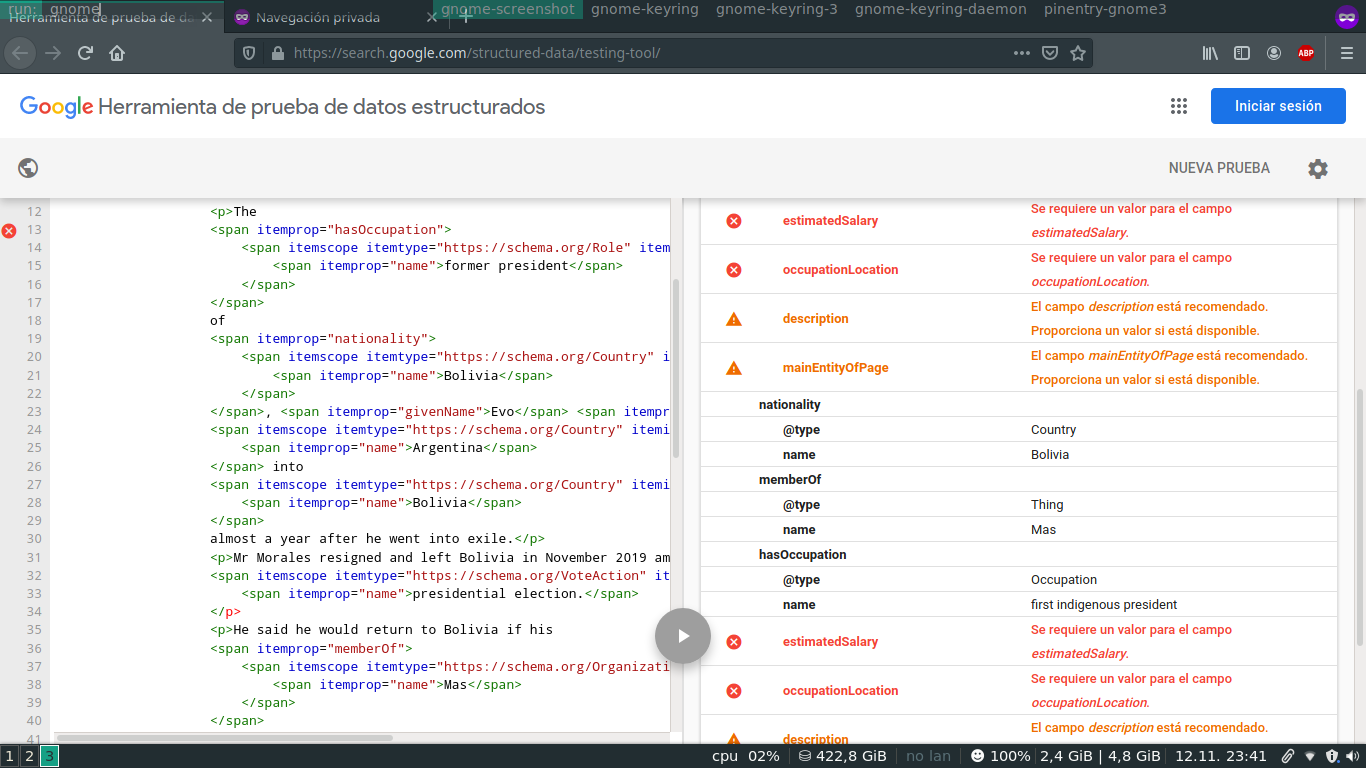
\includegraphics[width=\textwidth]{validacion-ex1}
\end{figure}

% Ejercicio 2
\section{Ejercicio 2}
En el ejercicio 2 hacemos una serie de mejoras en el fichero \textit{json-ld} disponible en \cite{jsonv3} y junto al contenido de \cite{microdata} despojado de microdatos creamos un documento HTML llamado \textit{exercise2.html}.
% Bibliografía
\begin{thebibliography}{8}
\bibitem{bbcevomorales}
Noticia de la BBC sobre el retorno del expresidente Evo Morales a Bolivia, \url{https://www.bbc.com/news/world-latin-america-54872827}. Última vez accedido 12 de noviembre de 2020.

\bibitem{permidtool}
\textit{Intelligent Tagging Demo}, herramienta de \textit{PermID}, \url{https://permid.org/onecalaisViewer}. Última vez accedido 12 de noviembre de 2020.

\bibitem{wikidata}
Página de la \textit{Wikidata}, \url{https://www.wikidata.org/wiki/Wikidata:Main_Page}. Última vez accedido 12 de noviembre de 2020.

\bibitem{googlesdtt}
Página de la \textit{Google Structured Data Testing Tool}, \url{https://search.google.com/structured-data/testing-tool/}. Última vez accedido 12 de noviembre de 2020.

\bibitem{jsonv3}
Página de Daniel Gayo-Avello donde encontramos el fichero \textit{json-ld}, \url{http://danigayo.info/ejemplos-SIW/03-json-ld-v3.json}. Última vez accedido 12 de noviembre de 2020.

\bibitem{microdata}
Página de Daniel Gayo-Avello donde encontramos el documento HTML con microdatos incrustados, \url{http://danigayo.info/ejemplos-SIW/microdata.html}. Última vez accedido 12 de noviembre de 2020.
\end{thebibliography}
\end{document}

